% VQ-VAE pipeline with straight-through estimator — TikZ source. Compiles to a
% tight standalone PDF (pdflatex figures/vq-pipeline.tex), which
% `book-scaffold build-figures` converts to public/figures/vq-pipeline.svg.
%
% Forward (solid): x -> encoder -> z_e -> quantize -> z_q -> decoder -> xhat.
% Backward (dashed): reconstruction gradient is copied AROUND the quantizer
% straight onto the encoder, because the STE backward Jacobian is the identity.
\documentclass[tikz,border=3pt]{standalone}
\usepackage{amsmath}
\usepackage{amssymb}
\usepackage{tikz}
\usetikzlibrary{positioning,arrows.meta,calc}
\begin{document}
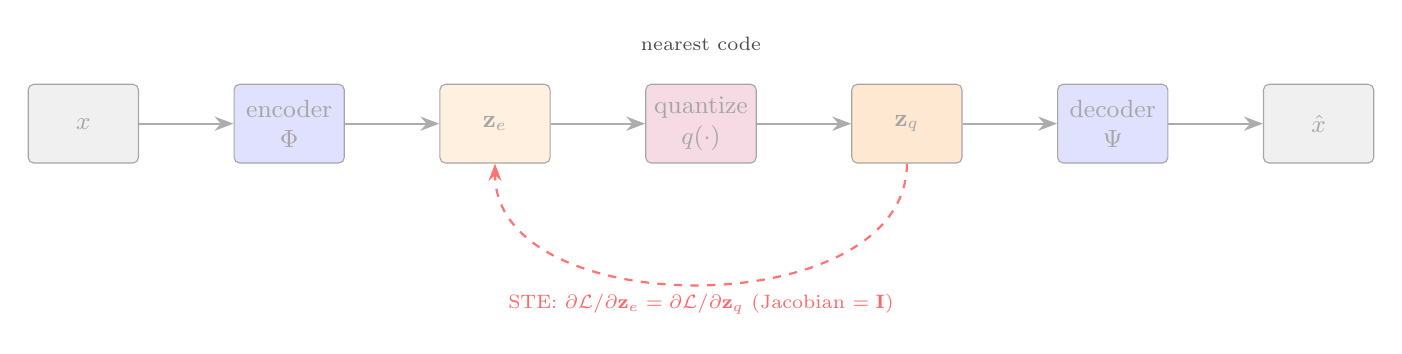
\begin{tikzpicture}[
    font=\small,
    box/.style={draw, gray!70, rounded corners=2pt, align=center,
                minimum height=10mm, minimum width=14mm, inner sep=3pt},
    fwd/.style={->, >={Stealth[length=2.4mm]}, gray!65, thick},
    bwd/.style={->, >={Stealth[length=2.2mm]}, red!55, thick, dashed},
  ]
  \node[box, fill=black!6] (x) {$x$};
  \node[box, fill=blue!12, right=12mm of x] (enc) {encoder\\$\Phi$};
  \node[box, fill=orange!12, right=12mm of enc] (ze) {$\mathbf z_e$};
  \node[box, fill=purple!14, right=12mm of ze] (q) {quantize\\$q(\cdot)$};
  \node[box, fill=orange!18, right=12mm of q] (zq) {$\mathbf z_q$};
  \node[box, fill=blue!12, right=12mm of zq] (dec) {decoder\\$\Psi$};
  \node[box, fill=black!6, right=12mm of dec] (xh) {$\hat x$};

  \draw[fwd] (x) -- (enc);
  \draw[fwd] (enc) -- (ze);
  \draw[fwd] (ze) -- (q);
  \draw[fwd] (q) -- (zq);
  \draw[fwd] (zq) -- (dec);
  \draw[fwd] (dec) -- (xh);

  % STE backward copy: from z_q back to z_e, bypassing q
  \draw[bwd] (zq.south) to[out=-90,in=-90] node[below, font=\scriptsize, text=red!60]
    {STE: $\partial\mathcal L/\partial\mathbf z_e=\partial\mathcal L/\partial\mathbf z_q$ (Jacobian $=\mathbf I$)} (ze.south);

  \node[above, font=\scriptsize, text=black!70] at ($(q.north)+(0,3mm)$)
    {nearest code};
\end{tikzpicture}
\end{document}
